\section{Commits}\label{sec:commits}

\begin{frame}
    \slidehead
    \begin{itemize}
        \item Datei hinzugefügt, geändert, verschoben oder gelöscht
        \item mit Nachricht versehen
        \item \enquote{kryptische} Bezeichnung (Hash), z.B. \texttt{bc7f1a9e22bc7f19e22bc}\dots
        \begin{itemize}
            \item erste fünf Zeichen zur Identifizierung meist ausreichend
        \end{itemize}
    \end{itemize}
\end{frame}

\begin{frame}
    \slidehead
    \vspace{-1em}
    \centering
    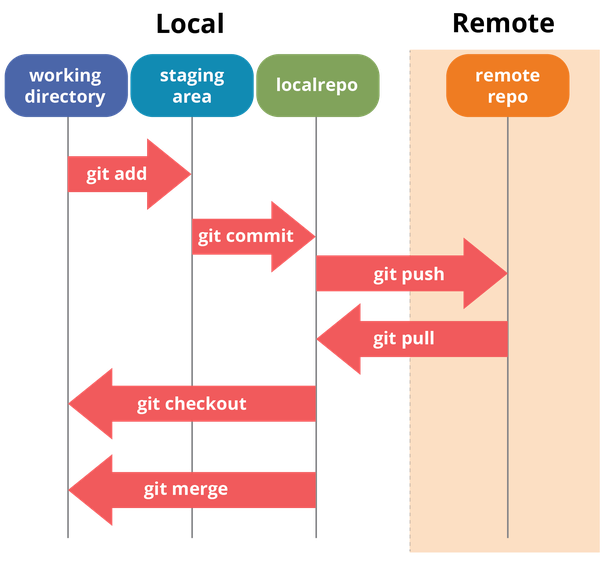
\includegraphics[scale=.3]{../pictures/structure-overview}
\end{frame}

\begin{frame}
    \slidehead
    \vspace{1em}
    \centering
    \begin{tikzpicture}
        % state 1
        \node[commit](c1){c1c1c};
        \node<1>[head, below=2 em of c1](head0){};
        \draw<1>[parent] (head0) to (c1);
        % state 2
        \node<2->[commit, right=2 em of c1](c2){c2c2c};
        \draw<2->[parent] (c2) to (c1);
        \node<2>[head, below=2 em of c2](head1){};
        \draw<2>[parent] (head1) to (c2);
        % state 3
        \node<3->[commit, right=2 em of c2](c3){c3c3c};
        \draw<3->[parent] (c3) to (c2);
        \node<3>[head, below=2 em of c3](head2){};
        \draw<3>[parent] (head2) to (c3);
        % state 4
        \node<4->[branch, below=2em of c3](branch_master){master};
        \draw<4->[parent] (branch_master) to (c3);
        \node<4>[head, below=2em of branch_master](head2){};
        \draw<4>[parent] (head2) to (branch_master);
        % state 5
        \node<5->[head, below=2em of c2](head2){};
        \draw<5->[parent] (head2) to (c2);
    \end{tikzpicture}
    \vspace{1em}\par
    \only<1>{initialer Commit \texttt{c1c1c}, z.B. \texttt{"initial commit"}}
    \only<2>{Commit \texttt{c2c2c}, z.B. \texttt{"implement add and mul"}}
    \only<3>{Commit \texttt{c3c3c}, z.B. \texttt{"fix sum"}}
    \only<4>{\texttt{HEAD} zeigt \textit{indirekt} auf einen Commit (hier \texttt{c3c3c})}
    \only<5>{\texttt{HEAD} kann auch \textit{direkt} auf Commit (hier \texttt{c2c2c}) zeigen}
\end{frame}
